\newpage
\section{\ac{SVAR} Identification} \label{SVARIdentification}

For implementaiton of the methods introduced in previous section the SVAR package in R \footcite[See.][]{Lange2020} software is used.
\subsubsection{SVAR Model Identification}
The structural VAR models are often used to trace the contemporaneous linkage among macroeconomic variables. The SVAR model has the following general form  \footcite[See.][]{Lange2020}: 
\[ A_0 Y_t = mu+  A_1(L) Y_t + B \epsilon_t \]
where yt = [y1t
, ..., yKt]
 is a vector of observable variables, Ai
, i = 1, . . . , p, are (K × K)
coefficient matrices, and intercept parameters are collected in µ. We focus on the case of time
invariant deterministic terms for notational clarity. Model augmentation with time-varying
deterministic terms (e.g., breaks, linear trends), however, is straightforward. Furthermore,
the VAR model is stationary (invertible) by assumption. The vector ut consists of reducedform residuals, which are serially uncorrelated with E(ut) = 0 and Cov(ut) = sigmau. The
nonsingular matrix B captures the instantaneous effects of the structural shocks
on the variables of the system
 Where $Y_t$ is n-vector relevant variables, then $A_0$ and $B$ are $n * n$ matrices and $A_1(L) = \sum\limits_{i=1}^ qA_{1i} L^i $ is the matrices polynomial in the lag operator in which $A$ matrices have the same size as $A_0$ matrix. The error terms$\epsilon_t$ (structural schocks) is an n-vector of serially uncorrelated zero mean structural schocks with and identitiy contemporanous covariance matrix. The crucial part in SVAR modelling is the choice of the macroeconomics variables. The second challenge is that the nmuber of parameters to be identified in the structural model is larger than that of the reduced VAR form. Therefore, some new relations needs to be introduced. This can be usually done by introducing restrictions on $A_0$ or $B_0$ matrix. 

In this work, we assume the following set of variables as the variables involed in modeling. 
The assumed $Y$ is :
\[ 
 \begin{bmatrix}
        ry \\ 
        \pi \\
        rg \\
        r \\
        mc \\
        h \\
        hp \\
  \end{bmatrix}
\]


\[ 
h^s = a_1 mc + a_2 rhp + b_1^s \epsilon^s
h^d = a_3 ry + a_4 rhp + a_5 r + a_6 \pi + a_7 rg  + b_1^d \epsilon^d
h^s = h^d
\]
The notion of time is deleted from the above equation but once can consider that the every variable reperesnt different time instance for example $a-1 mc$ depending on the cohsen number of lags represent $a_{1t} mc_{t} ,  a_{1(t-1)} mc_{(t-1)} ...  $
this will lead to 
\[
 rhp  = c_1 mc+  c_2 ry + c_3 rhp  + c_4 r + c_5 \pi + c_6 rg  + b_1 \epsilon
\]

The second assumption chosen by author in this work is that $A_0$ is a lower triangular matrix therefore as one can see in the order of variables in bla equation every variable can have only correlation with previous variables in the same time stamp and with all variable in previous time stamps. Therefore, the order of variables play a crucial role in our model. 


\subsection{\ac{SVAR} Results}
The following picture shows the impulse response of the identified model to different shocks. As one can see in Figure \ref{imp1}, when the housing supply increases housing price starts to decrease. This result fits to what we expected from the monetary transition channels. However, the plot shows a small drop in house price as a result of an increase in material cost. In my opinion, this is due to negligible affect of material cost on housing price in Germany. 
Furthermore, a close look at Figure \ref{imp2} show that after an increase in interest rate, housing price start to decrease for a period of 2 years. This result can also be explained with both IS-LM and Transition Channels model. the housing supply increases housing price starts to decrease. This result fits to what we expected from the monetary transition channels. Besides that, the plots implies that an increase in GDP leads to higher prices. This is also expected from an economy with growing GDP to experience and increase in house prices. However, the first plot implies that an increase in government spending can decrease the house price. In my opinion, this is not a result that one may expect. Usually an increase in government spending should lead to an increase in GDP and consequently the housing price. This impulse response can be a result of small number of lags (2 lags) chosen for the identified model and the sticky nature of housing price. Besides that, as the data set used for this identification covers only last 20 years,it can be that the data is not informative enough for this type of identification. However, this can be improved by adding feasibility constraints to the model. 
\begin{figure}[H]
\label{imp1}
\caption{Impulse Response of a Shock in Housing Supply, Housing Price and Material Cost on Housing Price}
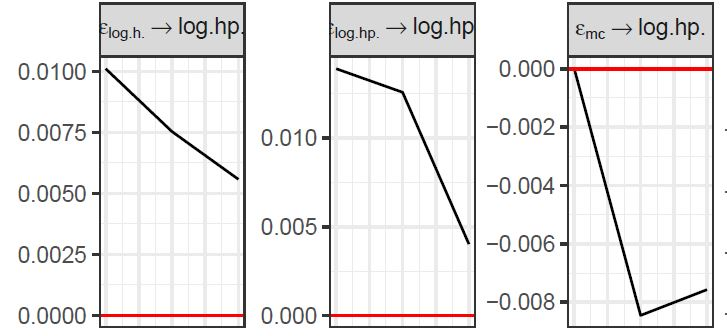
\includegraphics[width=0.9\textwidth]{hp1}
\\
Source: Own Graph
\end{figure}
\begin{figure}[H]
\label{imp2}
\caption{Impulse Response of a Shock Government Spending, Interest Rate and Output on Housing Price}
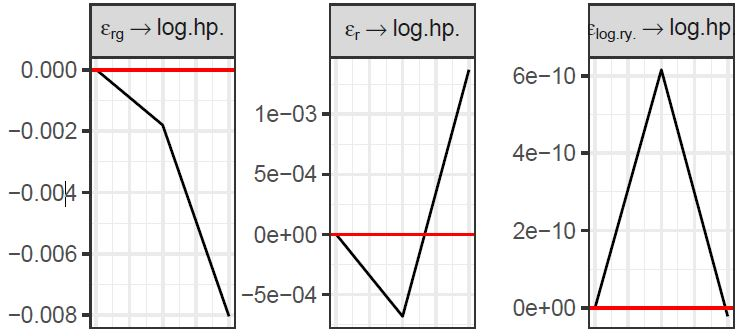
\includegraphics[width=0.9\textwidth]{hp2}
\\
Source: Own Graph
\end{figure}


